\newcommand{\source}[1]{\caption*{Source: {#1}} }

\section{Grundlagen}\raggedbottom

\subsection{Magen-Darmtrakt}
?? 

\subsection{CNN}
?? 

\subsection{U-Net}
% CNN, Convolution, Maxpooling oder ReLu erklären? 

U-Net wurde im Jahr 2015 von Olag Ronneberger et al. vorgestellt als Segmentierungsarchitektur für den biomedizinischem Bereich und bildet die Baseline dieser Arbeit. Klassisch handelt es sich um ein Convolutional Neural Network  bestehend es aus 5 bis 6 'downsampling' (auch Encoder genannt) Schichten und der gleichen Menge an "upsampling" (auch Decoder genannt) Schichten. 

Eine 'downsample' Operation besteht zum einen aus einer 'Convolution operation'  sowie einer 'Max pooling operation' an deren Ende jeweils eine ReLu Aktivierungsfunktion zum Einsatz kommt. In diesem Schritt lernt das Modell Eigenschaften auf Pixelebene, wie zum Beispiel Formen, Ecken, Kanten. Hierbei halbieren sich die Eingabedimensionen und die Tiefe des Bildes wird erhöht. 

Im Decoder wird das Bild wieder auf seine ursprüngliche Größe mittels 'Transpose Convolution operations' auf seine ursprüngliche Größe gebracht. Hier ersetzt die transponier Operation die Maxpooling Operation (vergleich Grafik). Dieser Part erlaubt dem Modell das lokalisieren der zuvor gelernten Eigenschaften und gibt eine Maske zurück für jede Klasse, in der 0 der Hintergrund ist und 1 die jeweilige Klasse. 

\subsection{RLE}
?

\section{Verwandte Arbeiten}\raggedbottom
2 Seiten dazu

\subsection{Semantische Segmentierung im medizinischem Bereich}

\subsection{Intelligentes Zuschneiden des Inputs}
Paper dazu ist da

\subsection{Loss Functions für Segmentierungsarchitekturen}
Paper dazu ist auch da

\subsection{Encoder 1}
Eventuell

\subsection{Encoder 2}
Eventuell

\section{Methodik}\raggedbottom

\subsection{Datenanalyse}
Der Datensatz besteht aus 115 488 Zeilen und enthält drei features: ID, Klasse und einem Run-lenght codierten String, der die Maske enthält. \autoref{tabelle_daten}. Jeder ID sind drei Zeilen gewidmet, jeweils für die drei Klassen. Zu jeder ID existiert ein Graustufen Bild, welche sich im train Ordner befinden: 

input\textbackslash uw-madison-gi-tract-image-segmentation\textbackslash train\textbackslash case101\textbackslash \\case101\textunderscore 
day20\textbackslash scans\textbackslash slice\textunderscore 0001\textunderscore 266\textunderscore 266\textunderscore 1.50\textunderscore 1.50.png

Jedes slice enthält vier Zahlen (z.B. 266\textunderscore 266\textunderscore 1.50\textunderscore 1.50.png), die ersten beiden stehen für die Auflösung des Bildes und die letzten beiden für den physischen Abstand der Pixel. Der Großteil der Aufnahmen stammt von Tag null oder tag eins \autoref{Fig:slice_per_day} und die durchschnittliche Anzahl an Bildern pro Fall beträgt X.

Beim betrachten der Verteilung der Segmentierungen fällt auf, dass das Vorkommen für jede Klasse stark variiert. \autoref{Fig:klassenverteilung}.

\begin{table}[]
	\begin{center}
		\begin{tabular}{lllll}
			\hline
			Index  & ID & Class & Segmentation \\
			\hline \hline
			1     & case134\textunderscore day0\textunderscore slice\textunderscore 0085 	& large\textunderscore bowel 	&  NaN  \\
			2     & case134\textunderscore day0\textunderscore slice\textunderscore 0085 	& small\textunderscore bowel 	&  41591 5 41599 7 41949 27 ...  \\
			3     & case134\textunderscore day0\textunderscore slice\textunderscore 0085 	& stomach 	&  NaN \\
			4     & case123\textunderscore day0\textunderscore slice\textunderscore 0001 	& large\textunderscore bowel 	&  35223 6 74352 7 32312 12 ...   \\
			5     & case123\textunderscore day0\textunderscore slice\textunderscore 0001 	& small\textunderscore bowel 	&  63432 5 12354 7 41949 12 ...  \\
			6     & case123\textunderscore day0\textunderscore slice\textunderscore 0001 	& stomach 	&  NaN \\
			\hline
		\end{tabular}
		\caption{Beispieldaten für zwe slices}\label{tabelle_daten}
	\end{center}
\end{table}

\begin{figure}[!htb]
   \begin{minipage}{0.48\textwidth}
     \centering
     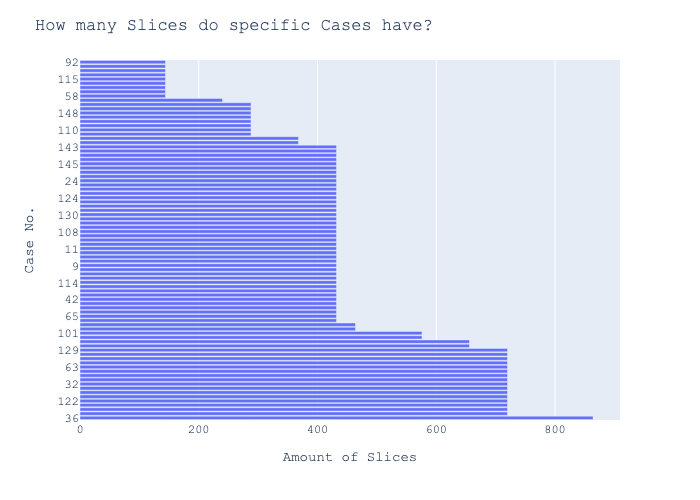
\includegraphics[width=1.2\linewidth]{bilder/slice_per_case}
     \caption{Anzahl Bilder pro Fall}\label{Fig:slice_per_case}
   \end{minipage}\hfill
   \begin{minipage}{0.48\textwidth}
     \centering
     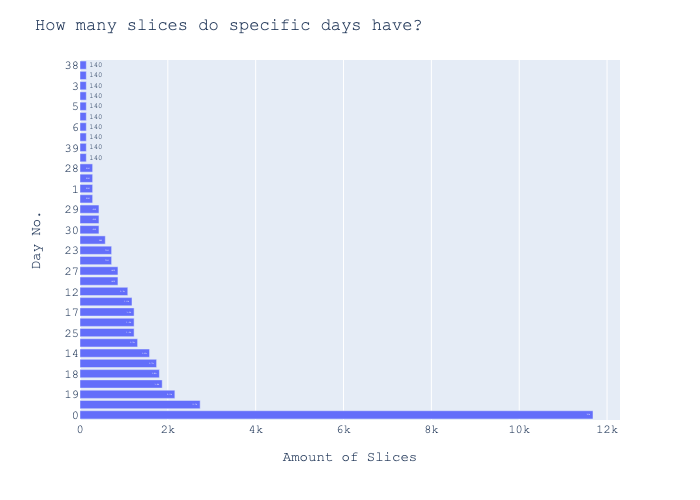
\includegraphics[width=1.2\linewidth]{bilder/slices_per_day}
     \caption{Anzahl Bilder pro Tag}\label{Fig:slice_per_day}
   \end{minipage}
\end{figure}

\subsection{Metadatenextraktion}




\subsection{Algorithmik}
?

\subsection{2.5 dimensionale Daten}
?

\subsection{Intelligentes Zuschneiden}
?

\subsection{Nachbearbeitung }
?

\subsection{Experimente}
Experimente.

\section{Evaluation}\raggedbottom

\section{Fazit}\raggedbottom

\subsection{Ausblick}
Ideen, die es nicht in die Arbeit geschafft haben oder nicht schafffen konnten.


\ifthenelse{\boolean{\biber}}{ % Beispiel um mit Biber zu zitieren (\citet und \citep)
	\citet{Con97} hat ein Buch geschrieben. Es gibt auch andere Arbeiten \citep{PeHe97} die referenziert sind. In Abbildung \ref{fig_Gallien} ist ein Sachverhalt dargestellt.


	1 Autor: \citet{Con97} \hspace*{1cm} \citep{Con97}\\
	2 Autoren: \citet{IWNLP} \hspace*{1cm} \citep{IWNLP}\\
	3 Autoren: \citet{liebeck-esau-conrad:2016:ArgMining2016} \hspace*{1cm} \citep{liebeck-esau-conrad:2016:ArgMining2016}

	Online resource: \citet{ILSVRC2016}
}{ %  Beispiel um klassisch zu zitieren (\cite)
	\cite{Con97} hat ein Buch geschrieben. Es gibt auch andere Arbeiten \cite{PeHe97} die referenziert sind. In Abbildung \ref{fig_Gallien} ist ein Sachverhalt dargestellt.


	1 Autor: \cite{Con97} \hspace*{1cm} \cite{Con97}\\
	2 Autoren: \cite{IWNLP} \hspace*{1cm} \cite{IWNLP}\\
	3 Autoren: \cite{liebeck-esau-conrad:2016:ArgMining2016} \hspace*{1cm} \cite{liebeck-esau-conrad:2016:ArgMining2016}

	Online resource: \cite{ILSVRC2016}
}

\ifthenelse{\equal{\sprache}{deutsch}}{
	\textbf{quotes}:\\
	Ein Beispiel für deutsche Anführungszeichen \glqq quote\grqq.
}{}

\begin{figure}[htb]
	\begin{center}
		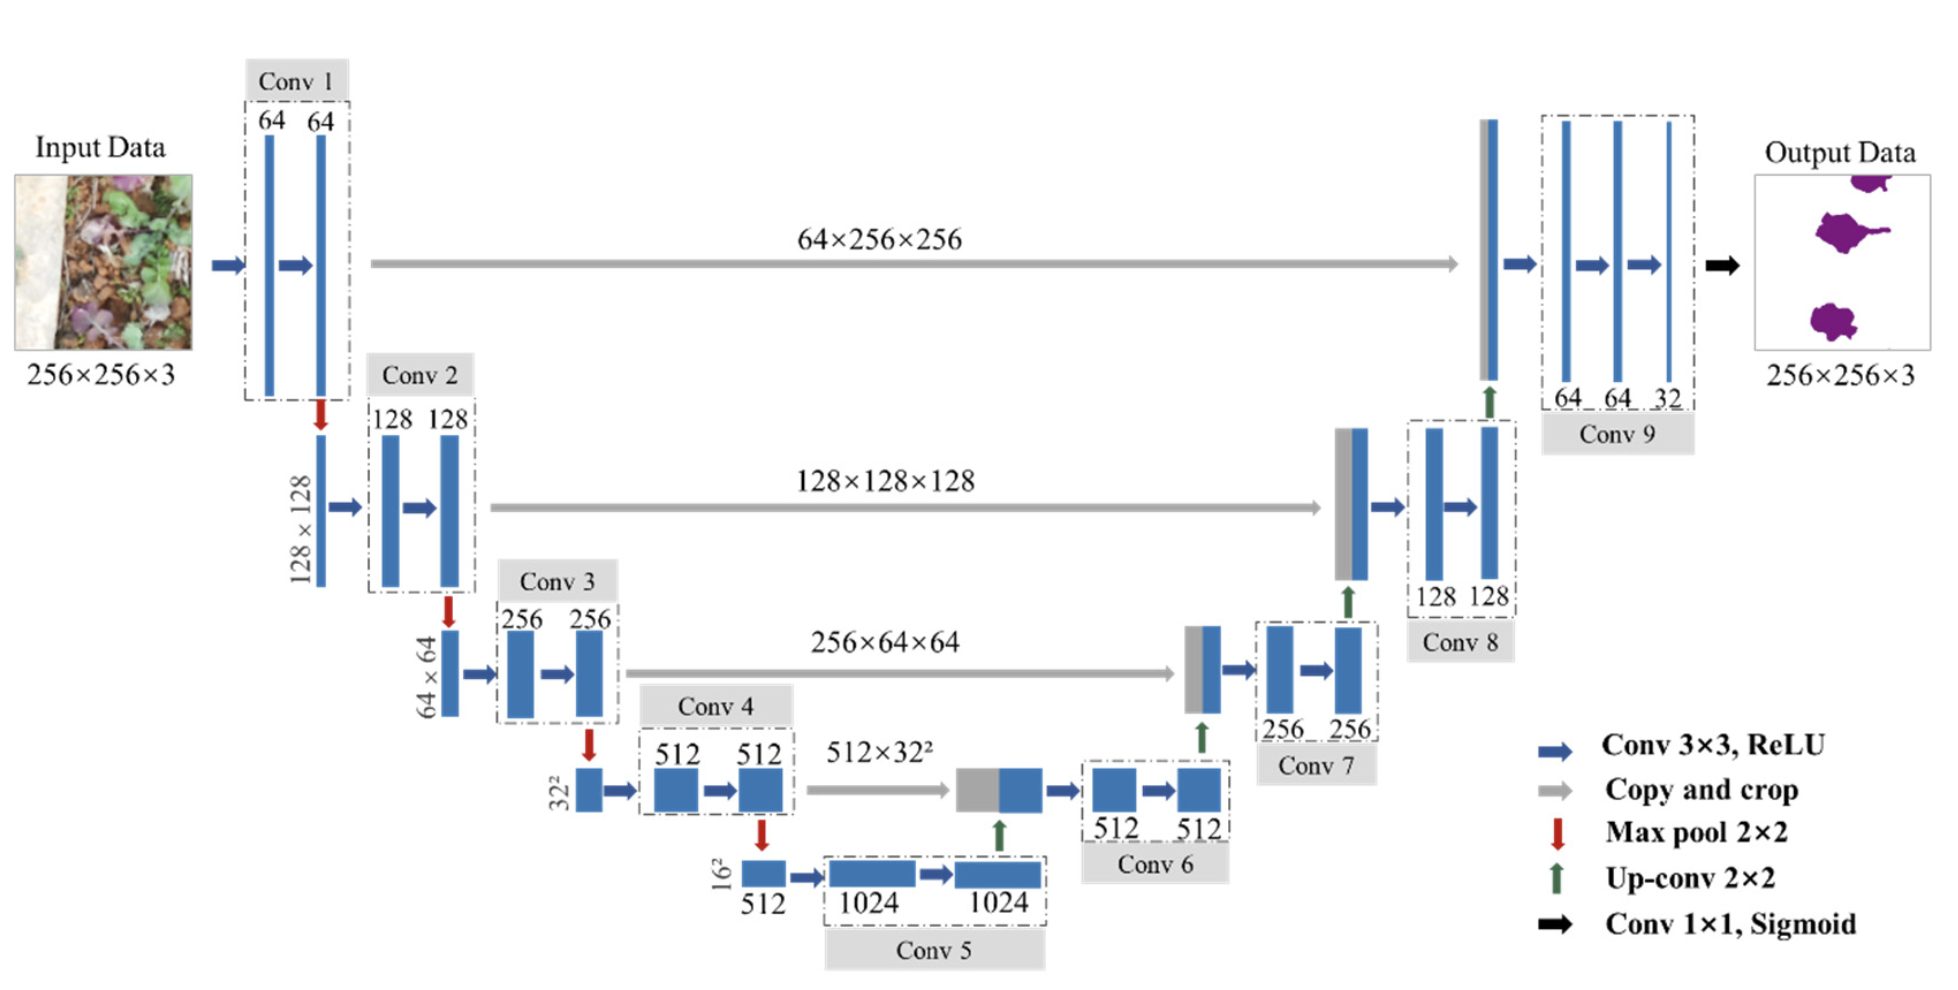
\includegraphics[width=300pt, angle=270]{bilder/u-net-architecture}
		\caption{U-Net Architektur}\label{Fig:unet-diagram}
	\end{center}
\end{figure}

\begin{figure}[htb]
	\begin{center}
		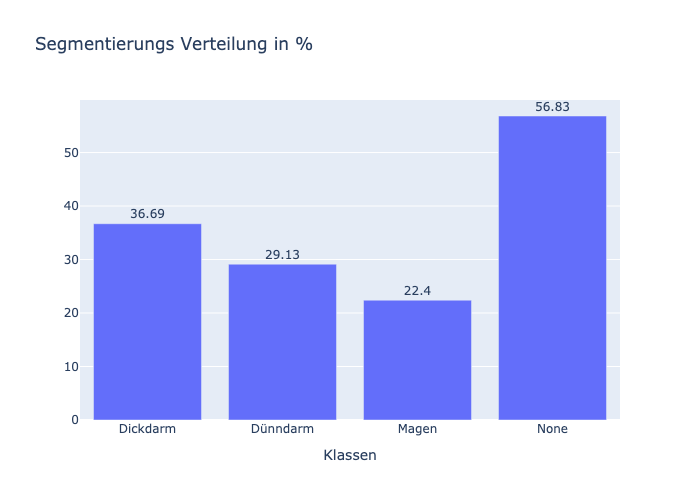
\includegraphics[width=220pt , angle=270]{bilder/segmentation_distribution}
		\caption{Verteilung der Klassen im Testset}\label{Fig:klassenverteilung}
	\end{center}
\end{figure}

\begin{figure}[htb]
	\begin{center}
		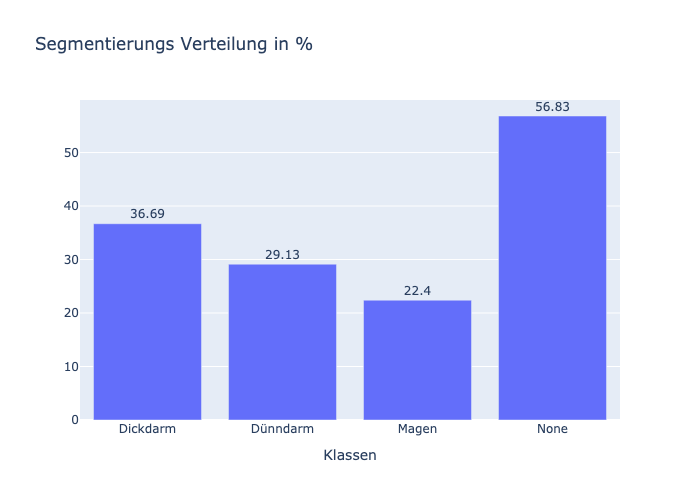
\includegraphics[width=220pt , angle=270]{bilder/segmentation_distribution}
		\caption{Verteilung der Klassen im Testset}\label{Fig:klassenverteilung}
	\end{center}
\end{figure}

\pagebreak